\chapter{\textit{Deployment} del nuovo sistema informatico}\label{ch:implementazione}

In questo capitolo viene descritta la pianificazione per la gestione del deployment della soluzione proposta da \azienda.


Vengono quindi individuate le attività principali e, per ciascuna di queste, vengono definiti dei \textit{task}.
Tali attività sono strettamente collegate con gli obiettivi presenti nella Sez. \ref{sec:obiettivi_helpdesk}~in quanto sono svolte al fine di soddisfare questi ultimi.

\section{Descrizione dell’implementazione}\label{sec:desc_implementazione}

	Per la transizione dal sistema informatico corrente a quello nuovo, \azienda~ha deciso di utilizzare totalmente il tempo di sei mesi fornito dal proponente.
	
	Dopo un'attenta analisi, \azienda~ha optato di effettuare un \rollout~con la tipologia \textit{Verticale}, scartando dnuque quella \textit{Orizzontale}.
	Questo in quanto, vista la suddivisione dell'azienda ospedaliera in multipli reparti, che possiamo definire modulari, risulta più conveniente e meno propenso ad errori, permettendo inoltre di adattare e testare facilmente il nuovo sistema in corso d'opera.
	
	\begin{figure}[h!]
		\centering
		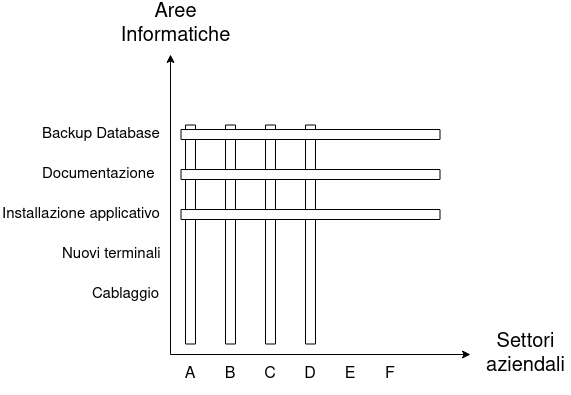
\includegraphics[width=\linewidth]{img/implementazione.png}
		\caption{Implementazione verticale \textit{vs} implementazione orizzontale}
		\label{fig:implementazione}
	\end{figure}

	In Fig. \ref{fig:implementazione}~è possibile vedere rappresentata in un grafico la differenza principale tra implementazione verticale, che appunto viene svolta in successione per ciascun settore aziendale, e quella orizzontale, che prevede implementare la feature in un unico momento in ciascun settore.

\newpage
\subsection{Implementazione Orizzontale}

	Un'implementazione orizzontale consiste nell'effettuare il passaggio da un sistema ad un altro in tutta l'azienda in una singola transizione.
	Questo approccio porta alcuni vantaggi, quali:
	\begin{itemize}[noitemsep]
		\renewcommand\labelitemi{--}
		\item tempo totale di transizione e implementazione più brevi;
		\item non ci possono essere due sistemi diversi utilizzati contemporaneamente all’interno dell’azienda;
		\item non sono presenti dispositivi che fungono da traduttori tra un sistema e un altro;
		\item è possibile concentrare le risorse esclusivamente per l'implementazione del nuovo sistema e non alla creazione di interfacce o fix per il sistema uscente;
		\item minori costi complessivi, essendo che il vecchio sistema viene dismesso più in fretta.
	\end{itemize}
	
	Tuttavia, sono presenti anche alcuni svantaggi, come ad esempio:
	\begin{itemize}[noitemsep]
		\renewcommand\labelitemi{--}
		\item impossibilità di eseguire un roll-back affidabile nel lungo periodo, dopo la dismissione del vecchio sistema;
		\item cambiamento improvviso del workflow lavorativo dei dipendenti e una conseguente diminuzione temporanea di produttività.
	\end{itemize}

\subsection{Implementazione Verticale}

	L'implementazione verticale è un approccio che effettua una transizione graduale ed uniforme del sistema all'interno dell'azienda.
	
	Per questa tipologia di \rollout~i vantaggi sono:
	\begin{itemize}[noitemsep]
		\renewcommand\labelitemi{--}
		\item un adattamento più chiaro e veloce al nuovo sistema informatico;
		\item problemi e difficoltà di implementazione possono essere scoperte prima che tutta l'azienda ne sia affetta, ma solamente una singola area, e quindi risolti in maniera graduale;
		\item la loro produttività resta inalterata grazie al cambio graduale;
	\end{itemize}

	Come per l'implementazione orizzontale, anche quella verticale presenta alcuni svantaggi, quali:
	\begin{itemize}[noitemsep]
		\renewcommand\labelitemi{--}
		\item costi di implementazione più alti a causa, tra cui, della coesistenza parziale di due sistemi;
		\item presenza di interfacce per la comunicazione tra un sistema e un altro;
		\item periodo prolungato di formazione;
		\item difficoltà di integrazione dei due sistemi.
	\end{itemize}

\section{Fasi dell'implementazione}

	Dopo un'attenta lettura del capitolato, le fasi definite per l'implementazione del nuovo sistema sono:
	\begin{enumerate}
		\item \textbf{Definizione del nuovo \helpdesk}
			\begin{itemize}[noitemsep]
				\renewcommand\labelitemi{--}
				\item Identificazione, discussione e approvazione dei moduli;
				\item Identificazione delle eventuali estensioni al progetto;
				\item Identificazione delle eventuali personalizzazioni al progetto;
				\item Identificazione dei requisiti della soluzione e dei criteri di soddisfacimento.
			\end{itemize}
			
		\item \textbf{Sviluppo del nuovo \helpdesk}
			\begin{itemize}[noitemsep]
				\renewcommand\labelitemi{--}
				\item Realizzazione di mockup e PoC dei servizi principali del nuovo sistema;
				\item Definizione di eventuali estensioni a tali servizi;
				\item Implementazione delle estensioni richieste;
				\item Realizzazione e presentazione di un prototipo;
				\item Completamento del prototipo e test;
				\item Realizzazione di documentazione tecnica ed altro materiale per gli utenti.
			\end{itemize}
			
		\newpage
		\item \textbf{Installazione per area}
			\begin{itemize}[noitemsep]
				\renewcommand\labelitemi{--}
				\item Installazione delle soluzioni su ambienti di produzione, di sviluppo e di test per ciascuna delle aree dell'istituto definite nel capitolato d'appalto;
				\item Configurazione delle soluzioni in base alle necessità definite precedentemente;
				\item Impostazione dei profili utente e assegnazione dei privilegi;
				\item Importazione dei dati necessari al funzionamento della nuova soluzione.
			\end{itemize}
		
		\item \textbf{Formazione dei dipendenti dell'\istituto~sul nuovo sistema}
			\begin{itemize}[noitemsep]
				\renewcommand\labelitemi{--}
				\item Affiancamento di \azienda~al \proponente~per fornire formazione agli utenti del nuovo sistema;
				\item Adeguamento della documentazione e dei manuali utente.
			\end{itemize}
		
		\item \textbf{Installazione per area del nuovo sistema in produzione}
			\begin{itemize}[noitemsep]
				\renewcommand\labelitemi{--}
				\item Per ciascuna area, l'\istituto, dopo aver validato che siano stati implementati tutti i requisiti, autorizza \azienda~a procedere al passaggio dal vecchio al nuovo sistema;
				\item Trasferimento dei dati dal vecchio al nuovo sistema;
				\item Freeze del vecchio sistema in caso di \rollback;
			\end{itemize}
		
		\item \textbf{Affiancamento dei dipendenti in vista della riconsegna}
			\begin{itemize}[noitemsep]
				\renewcommand\labelitemi{--}
				\item Affiancamento da parte di \azienda~verso l'\istituto~nel primo periodo di utilizzo del nuovo sistema;
				\item Eventuale perfezionamento della documentazione;
				\item Risoluzione di eventuali bug e perfezionamento del sistema (tramite piccole modifiche);
				\item Identificazione e risoluzione di incidenti e problemi;
				\item Successivamente, supporto da parte di \azienda~tramite il proprio Service Desk.
			\end{itemize}
		
	\end{enumerate}

	Le fasi numero tre, ``\textit{Installazione per area}'', e cinque, ``\textit{Go-live del nuovo sistema per area}'', rappresentano l'installazione e la messa in produzione del sistema in base a ciascuna delle aree ospedaliere presenti nel capitolato fornito dal \proponente.
	Questo in quanto viene effettuato un \rollout~con implementazione verticale, come spiegato in \ref{sec:desc_implementazione}.
	
	\subsection{Presa in carico del progetto}
	
		Come specificato nel capitolato fornito dall'\istituto, il \proponente~desidera passare da una fornitura con service provider multipli ad una fornitura di tipo ``\textit{sole provider}''.
	
		\azienda~si impegna dunque a prendere in carico la gestione di tutti i contratti esistenti alla data di aggiudicazione dell'appalto, contattando gli attuali fornitori e terminando i servizi in essere.
		Avvisare gli attuali fornitori è essenziale per una regolare e corretta presa in carico.
		
		In caso di irregolarità o incomprensioni, \azienda~avvertirà il Coordinatore di Progetto, allo scopo di prendere una decisione per risolvere la situazione.
	
	\subsection{Riconsegna del progetto}
	
		Come descritto da capitolato, \azienda si impegna a riconsegnare il progetto completo dopo nove anni passati dalla presa in carico.

		Verranno quindi consegnate le credenziali di accesso al sistema, tutta la documentazione prodotta, tutti i sistemi hardware e software comprati e prodotti durante la durata del progetto e tutte le risorse che erano state fornite ad \azienda~con lo scopo di completare il progetto descritto nel capitolato d'appalto.

\section{Attività principali}\label{sec:attivita_principali}

	In questa sezione vengono analizzate con maggiore attenzione alcune delle attività principali della fase di implementazione.
	Per ciascuna di queste vi sono cinque indicatori:
	\begin{itemize}[noitemsep]
		\renewcommand\labelitemi{--}

		\item \textit{Input}: i dati e le informazioni che vengono dati in input all'attività in maniera che questa funzioni correttamente;

		\item \textit{Deliverable} (o \textit{Output}): quello che viene prodotto dall'attività, potrebbero essere oggetti materiali o artefatti digitali;

		\item \textit{Risorse}: risorse necessarie dall'attività per trasformare l'input nell'output;

		\item \textit{Criteri di accettazione}: criteri, accordati tra \azienda~e proponente, che dicono quando un'attività è stata conclusa con successo; 

		\item \textit{Responsabili}: ruoli responsabili del corretto svolgimento dell'attività.
		
	\end{itemize}

	Inoltre, quando necessario, l'attività verrà suddivisa in compiti (tasks) aventi maggiore granularità.
	Successivamente, nella Sez. \ref{sec:pianificazione}, viene presentata una pianificazione di tali attività.
	
	Le attività di seguito presentate sono strettamente correlate con gli obiettivi elencati in \ref{sec:obiettivi_helpdesk}.
	
%	\newpage
	\subsection{Implementazione della nuova \textit{BPR}}\label{subsec:bpr_implmentation}

		L'attività di BPR tratta una profonda revisione dei processi aziendali, che, come spiegato in \ref{sec:desc_bpr}, si intende un intervento organizzativo di \textit{profonda revisione} dei procedimenti operativi.
		
		Tale attività può cominciare da subito in quanto prevede una lunga e profonda analisi del modello attuale dell'istituto
		
		\begin{itemize}[noitemsep]
			\renewcommand\labelitemi{--}
			\item \textbf{Input}: manuali e osservazioni del modello gerarchico attualmente in uso dall'azienda, ovvero analisi della situazione \textit{as-is};
			\item \textbf{Deliverable}: documento che descrive i nuovi processi creati in base alle necessità aziendali del proponente e documento che descrive le attività necessarie alla transizione dalla struttura gerarchica al nuovo sistema tramite BPR e l'implementazione di questo;
			\item \textbf{Risorse}: personale esperto in processi aziendali di \azienda~e personale dell'istituto che si occupa dell'organizzazione del modello gerarchico, ciascuno dotato di un proprio computer, adetto all'analisi dell'attuale modello e alla stesura dei nuovi processi aziendali;
			\item \textbf{Criteri di accettazione}: accettazione da parte del proponente dei nuovi processi stilati;
			\item \textbf{Responsabili}: analisti con conoscenza di processi aziendali.
		\end{itemize}
	
		\textbf{Tasks:}
		\begin{enumerate}[noitemsep]
			\item analisi dell'attuale modo di lavoro;
			\item stesura dei nuovi processi;
			\item approvazione di tali processi da parte del proponente.
		\end{enumerate}
	
		Gli obiettivi che questa attività è volta a soddisfare sono:
		\begin{itemize}[noitemsep]
			\renewcommand\labelitemi{--}
			\item {\color{pantone}IGP\_\ref{igp:1}}
			\item {\color{pantone}IGP\_\ref{igp:7}}
			\item {\color{pantone}IGP\_\ref{igp:8}}
			\item {\color{pantone}IGP\_\ref{igp:9}}
		\end{itemize}

%	\newpage
	\subsection{Scrittura della documentazione relativa al progetto}
	
		Come per l'attività precedente, anche quella riguardante la documentazione a una durata che parte dall'inizio del progetto fino alla sua conclusione.
		
		Avere una documentazione aggiornata e ben organizzata è inoltre alla base delle richieste da rispettare per perseguire certificazioni di standard, come richiesto appunto dall'\istituto~in {\color{pantone}IGP\_\ref{igp:7}}.
		
		\begin{itemize}[noitemsep]
			\renewcommand\labelitemi{--}
			\item \textbf{Input}: intero archivio della documentazione attuale riguardante il sistema informatico attualmente in uso e il sistema gerarchico;
			\item \textbf{Deliverable}: vengono forniti in output tutti i documenti riguardanti il progetto e la sua evoluzione;
			\item \textbf{Risorse}: per questa attività ciascuna delle persone coinvolte nel progetto dovrà dedicare tempo per documentare ciò che ha svolto;
			\item \textbf{Criteri di accettazione}: criteri quali chiarezza nella lettura e correttezza con quanto svolto verranno usati per validare il documento;
			\item \textbf{Responsabili}: i manager di ciascun gruppo saranno responsabili per la qualità della documentazione prodotta.
		\end{itemize}
		
		\textbf{Tasks:}
		\begin{enumerate}[noitemsep]
			\item ciascun dipendente pianifica le attività che deve svolgere;
			\item durante e dopo aver svolto tale attività, i dipendenti dovranno usare template forniti da \azienda~e concordati con l'\istituto, per documentare quanto svolto;
			\item riunioni a cadenza settimanale o bisettimanale, in base alle attività svolte, verranno usate per revisionare i documenti ed accettarli.
		\end{enumerate}
	
		Gli obiettivi che questa attività è volta a soddisfare sono:
		\begin{itemize}[noitemsep]
			\renewcommand\labelitemi{--}
			\item {\color{pantone}IGP\_\ref{igp:1}}
			\item {\color{pantone}IGP\_\ref{igp:7}}
			\item {\color{pantone}IGP\_\ref{igp:8}}
			\item {\color{pantone}IGP\_\ref{igp:9}}
			\item {\color{pantone}IGP\_\ref{igp:15}}
			\item {\color{pantone}IGP\_\ref{igp:17}}
		\end{itemize}

%	\newpage
	\subsection{\textit{Hand-off} dei sistemi ed erogazione dei servizi esistenti}
		
		La presa in carico dei sistemi esistenti da parte dell'offerente implica l'impegno di \azienda~ad erogare senza interuzioni i servizi che i precedenti fornitori offrivano.
		
		\begin{itemize}[noitemsep]
			\renewcommand\labelitemi{--}
			\item \textbf{Input}: documentazione e strumentazione relative a tutti i servizi attualmente in uso;
			\item \textbf{Deliverable}: continuativa erogazione dei servizi esistenti;
			\item \textbf{Risorse}: personale tecnico dell'istituto che possa spiegare e direzionare gli esperti di \azienda~per un corretto hand-off;
			\item \textbf{Criteri di accettazione}: erogazione dei servizi attuali senza interruzione;
			\item \textbf{Responsabili}: il responsabile della progettazione sarà colui che pianificherà la transizione in maniera che questa avvenga senza interruzioni.
		\end{itemize}
		
		\textbf{Tasks:}
		\begin{enumerate}[noitemsep]
			\item meeting di presentazione da parte dei tecnici di \azienda~e istituto nel quale vengono spiegati i sistemi attualmente in uso e quali servizi vengono erogati;
			\item ottenimento da parte dei tecnici di \azienda~delle credenziali e dei permessi necessari per poter accedere a tali sistemi e garantire una corretta erogazione;
			\item analisi delle logiche e delle modalità di erogazione dei servizi in uso;
			\item analisi e test dei servizi esistenti da parte dei tecnici di \azienda~insieme ai responsabili del proponente per assigurarsi di una corretta erogazione.
		\end{enumerate}
	
		Gli obiettivi che questa attività è volta a soddisfare sono:
		\begin{itemize}[noitemsep]
			\renewcommand\labelitemi{--}
			\item {\color{pantone}IGP\_\ref{igp:4}}
			\item {\color{pantone}IGP\_\ref{igp:5}}
			\item {\color{pantone}IGP\_\ref{igp:6}}
			\item {\color{pantone}IGP\_\ref{igp:12}}
			\item {\color{pantone}IGP\_\ref{igp:15}}
			\item {\color{pantone}IGP\_\ref{igp:16}}
			\item {\color{pantone}IGP\_\ref{igp:18}}
			\item {\color{pantone}IGP\_\ref{igp:19}}
		\end{itemize}

%	\newpage
	\subsection{Presa in carico postazioni di lavoro}
	
		Come elencato nel capitolato tecnico fornito dall'\istituto, le postazioni di lavoro dei dipendenti attualmente presenti sono molto diverse in quanto provvengono da fornitori diversi e dunque sono di marche e anni di acquisto diversi.
		Per certe postazioni alcuni di questi dati non sono disponibili.
		Tali contraddizioni sono la causa di un processo di \textit{Service Asset} e \textit{Configuration Management} svolti in maniera non ottimale.
		
		\azienda, come richiesto dal proponente, prende in carica la gestione di tali postazioni e garantisce di risolvere le problematiche riguardo il magazzino e di incongruenze nell'hardware.
		A tale scopo verrà istutuito un processo per controllare regolarmente le postazioni di lavoro.
		\azienda~si impegna inoltre di creare un sistema di magazzino in maniera da monitorare la presenza dei pezzi di ricambio con una granularità congrua alle necessità dell'\istituto.
		
		Attività di riorganizzazione come questa aiutano l'\istituto~a diventare eleggibile per certificazioni di standard e normative nazionali ed internazionali, come richiesto nell'obiettivo {\color{pantone}IGP\_\ref{igp:7}}.
		
		All'interno di questa attività vengono inclusi anche strumenti come stampanti e altro hardware che funge da periferiche per i computer.
		Come per i computer, anche tali dispositivi verranno registrati in magazzino e verranno forniti pezzi di ricambio, quando possibile.
		
		\begin{itemize}[noitemsep]
			\renewcommand\labelitemi{--}
			\item \textbf{Input}: lista completa dell'hardware presente all'interno dell'istituto, credenziali di accesso ai sistemi, privilegi necessari per poter installare nuovo hardware;
			\item \textbf{Deliverable}: sistemi uniformi in tutto l'istituto e un sistema di stoccaggio che permette di tracciare i pezzi in uso e gli eventuali pezzi di ricambio;
			\item \textbf{Risorse}: personale tecnico dell'istututo che indichi dove sono presenti i computer e altro hardware attualmente in uso;
			\item \textbf{Criteri di accettazione}: corretta integrazione dei nuovi computer e adeguata potenza in base alle necessità dei dipendenti e delle funzioni che devono svolgere;
			\item \textbf{Responsabili}: il responsabile alla progettazione e il responsabile alla privacy saranno incaricati della supervisione e della corretta esecuzione di tale attività.
		\end{itemize}
		
		\textbf{Tasks:}
		\begin{enumerate}[noitemsep]
			\item identificazione delle attuali postazioni di lavoro, e altro hardware, da sostituire;
			\item stipulazione di un contratto per l'acquisto di nuovo hardware, possibilmente con un grande magazzino o una casa madre;
			\item catalogazione nel magazzino e installazione del nuovo hardware;
			\item test e benchmark dei nuovi sistemi.
		\end{enumerate}

		Gli obiettivi che questa attività è volta a soddisfare sono:
		\begin{itemize}[noitemsep]
			\renewcommand\labelitemi{--}
			\item {\color{pantone}IGP\_\ref{igp:2}}
			\item {\color{pantone}IGP\_\ref{igp:3}}
			\item {\color{pantone}IGP\_\ref{igp:4}}
			\item {\color{pantone}IGP\_\ref{igp:6}}
			\item {\color{pantone}IGP\_\ref{igp:7}}
			\item {\color{pantone}IGP\_\ref{igp:11}}
			\item {\color{pantone}IGP\_\ref{igp:18}}
		\end{itemize}

%	\newpage
	\subsection{Revisione cablaggio e architettura di rete}\label{subsec:revisione_rete}
	
		Come descritto all'interno del capitolato fornito dall'\istituto, l'attuale architettura di rete presenta alcune problematiche, quali, ad esempio, tratti a bassa velocità, tratti che bypassano il centro stella, per collegarsi direttamente al centro elaborazione dati (o \textit{CED}).

		L'attuale organizzazione della rete ospedaliera rende tale centro stella un \textit{single point of failure} che mette a repentaglio l'intero sistema.
		Questo dovuto al fatto che non ci sono \textit{failover}, ovvero non vi sono sistemi secondari che possono subentrare in caso di malfunzionamenti.
		
		\azienda~si impegna dunque a riformare tale rete in maniera da renderla solida e sicura, assicurando dunque che non vi siano points of failure fatali e che, anche in caso di eventuali fallimenti, i dipendenti non si accorgano del downtime.
	
		Per fare ciò, può essere necessario l'acquisto di nuovi server o apparati di rete, anche dello stesso marchio e modello in maniera da facilitarne la manutenzione.
	
		\begin{itemize}[noitemsep]
			\renewcommand\labelitemi{--}
			\item \textbf{Input}: mappa della rete attuale, accesso alla strumentazione e all'hardware che forma la rete;
			\item \textbf{Deliverable}: una rete ristrutturata e solida insieme alla documentazione che ne spiega il partizionamento e il piano di indirizzamento; 
			\item \textbf{Risorse}: analisti e progettisti di rete e nuovo hardware;
			\item \textbf{Criteri di accettazione}: la nuova rete deve soddisfare tutti i requisiti del proponente per l'interconnessione dei computer e altro hardware. Tali requisiti vengono validati tramite test sulla ridondanza e sulle funzionalità di rete;
			\item \textbf{Responsabili}: progettisti di rete.
		\end{itemize}
		
		\textbf{Tasks:}
		\begin{enumerate}[noitemsep]
			\item analisi della rete attuale da parte di \azienda;
			\item stesura di un documento piano di indirizzamento IP e di partizionamento della rete;
			\item implementazione della nuova rete con eventuali nuovi server ed altri apparati di rete;
			\item convalida del nuovo sistema tramite test che ne possano verificare il corretto funzionamento e ridondanza.
		\end{enumerate}

		Gli obiettivi che questa attività è volta a soddisfare sono:
		\begin{itemize}[noitemsep]
			\renewcommand\labelitemi{--}
			\item {\color{pantone}IGP\_\ref{igp:2}}
			\item {\color{pantone}IGP\_\ref{igp:3}}
			\item {\color{pantone}IGP\_\ref{igp:4}}
			\item {\color{pantone}IGP\_\ref{igp:5}}
			\item {\color{pantone}IGP\_\ref{igp:6}}
			\item {\color{pantone}IGP\_\ref{igp:15}}
			\item {\color{pantone}IGP\_\ref{igp:16}}
		\end{itemize}
	
%	\newpage
	\subsection{Revisione del \textit{Centro Elaborazione Dati} (\textit{CED})}
		
		\azienda, vista la necessità di riprogettare il Centro Elaborazione Dati (o \textit{CED}) dell'\istituto, ha scelto di optare per una soluzione ibrida tra server in cloud e server \textit{in loco}, acquistati e tenuti localmente all'interno della struttura.
		
		Tale scelta è stata fatta in quanto una corretta integrazione tra cloud e locale facilita la manutenzione di operazioni come ad esempio i backup automatizzati e permette di avere meno possibili \textit{points of failure}, come accennato in \ref{subsec:revisione_rete} per il centro stella della rete.
		
		Il principale obiettivo che va ad essere soddisfatto da questa attività è {\color{pantone}IGP\_\ref{igp:19}}, nel quale l'\istituto~esprime il bisogno di una riorganizzazione dei locali CED presenti all'interno del sistema.
		
		\begin{itemize}[noitemsep]
			\renewcommand\labelitemi{--}
			\item \textbf{Input}: documentazione necessaria sui servizi attuali del CED, hardware e software (inclusi di codice sorgente ove presente) che compongono il CED, obiettivi e requisiti del nuovo CED;
			\item \textbf{Deliverable}: un nuovo CED aggiornato e \textit{ad-hoc} creato in base alle necessità dell'\istituto;
			\item \textbf{Risorse}: personale tecnico dell'\istituto~che affiancherà i dipendenti di \azienda~nella creazione del nuovo CED;
			\item \textbf{Criteri di accettazione}: per tale attività i criteri rappresentano i test di accettazione finali che stabiliranno se il nuovo CED rispetta tutti gli obiettivi e le richieste fatte dagli stakeholders;
			\item \textbf{Responsabili}: il responsabile della progettazione del nuovo sistema si occuperà di controllare che il proseguimento del lavoro sia in linea con quello che viene richiesto dall'istituto.
		\end{itemize}
		
		\textbf{Tasks:}
		\begin{enumerate}[noitemsep]
			\item presa in carico del sistema \textit{as-is} incluso di documentazione e affiancamento dei dipendenti di \azienda~da parte dei tecnici dell'\istituto~per una prima introduzione del sistema;
			\item implementazione del nuovo sistema in base ai requisiti decisi dal \proponente;
			\item esecuzione di test periodici per verificare la corretta implementazione del CED;
			\item riunioni periodiche con gli stakeholders per garantire che tutto venga implementato secondo le richieste;
			\item alla fine del progetto verranno eseguiti i test di accettazione e verrà riconsegnato il sistema con tutta la documentazione e deliverable che sono stati prodotti per la durata del progetto.
		\end{enumerate}

		Gli obiettivi che questa attività è volta a soddisfare sono:
		\begin{itemize}[noitemsep]
			\renewcommand\labelitemi{--}
			\item {\color{pantone}IGP\_\ref{igp:2}}
			\item {\color{pantone}IGP\_\ref{igp:3}}
			\item {\color{pantone}IGP\_\ref{igp:4}}
			\item {\color{pantone}IGP\_\ref{igp:5}}
			\item {\color{pantone}IGP\_\ref{igp:6}}
			\item {\color{pantone}IGP\_\ref{igp:7}}
			\item {\color{pantone}IGP\_\ref{igp:10}}
			\item {\color{pantone}IGP\_\ref{igp:14}}
			\item {\color{pantone}IGP\_\ref{igp:16}}
			\item {\color{pantone}IGP\_\ref{igp:19}}
		\end{itemize}

	\newpage
	\subsection{Implementazione del \textit{Centro di Gestione Integrato} (\textit{CGI})}
	
		L'istituto richiede inoltre la costituzione di un Centro di Gestione Integrato (o CGI), il quale sarà preliminare all'avvio dei nuovi servizi di gestione ed assistenza incluso l'Help Desk.
		Il principale obiettivo che questa attività va a soddisfare è {\color{pantone}IGP\_\ref{igp:21}}.
		
		Tale CGI ha come scopo quello di fornire un servizio dedicato di gestione e assistenza all'intera struttura ospedaliera.
		Secondo le richieste del capitolato, il CGI dovrà essere composto da:
		\begin{itemize}[noitemsep]
			\renewcommand\labelitemi{--}
			\item servizio di Help Desk;
			\item centro di controllo e monitoraggio
			\item servizi On-Site per le postazioni di lavoro
			\item reperibilità notturna e festiva del personale
			\item centro di Supporto per l'area direzionale
			\item centro di Supporto per l'area gestione personale
		\end{itemize}
	
		\begin{itemize}[noitemsep]
			\renewcommand\labelitemi{--}
			\item \textbf{Input}: requisiti e obiettivi del CGI che \azienda~si è fatta carico di progettare;
			\item \textbf{Deliverable}: CGI completo e funzionante;
			\item \textbf{Risorse}: per l'implementazione di tale CGI sarà necessario accedere ai dati aziendali raccolti fino a questo momento e ai workflow che stipulano come questi dati vengono gestiti;
			\item \textbf{Criteri di accettazione}: come per altri deliverable che compongono il progetto, anche il CGI ha come criterio il passaggio dei test di accettazione svolti con il \proponente.
			\item \textbf{Responsabili}: il responsabile della progettazione si occuperà di controllare e di portare a compimento l'implementazione di questo sottosistema.
		\end{itemize}
		
		\textbf{Tasks:}
		\begin{enumerate}[noitemsep]
			\item presa in carico del sistema \textit{as-is} e definizione dei requisiti per il CGI;
			\item implementazione del CGI in base ai requisiti definiti precedentemente;
			\item esecuzione di test periodici per verificarne la corretta implementazione;
			\item riunioni periodiche con gli stakeholders per garantire che tutto venga implementato secondo le richieste;
			\item svolgimento dei test di accettazionee e riconsegna del sistema insieme a documentazione ed altri eventuali deliverable.
		\end{enumerate}
	
		Gli obiettivi che questa attività è volta a soddisfare sono:
		\begin{itemize}[noitemsep]
			\renewcommand\labelitemi{--}
			\item {\color{pantone}IGP\_\ref{igp:1}}
			\item {\color{pantone}IGP\_\ref{igp:2}}
			\item {\color{pantone}IGP\_\ref{igp:3}}
			\item {\color{pantone}IGP\_\ref{igp:6}}
			\item {\color{pantone}IGP\_\ref{igp:7}}
			\item {\color{pantone}IGP\_\ref{igp:8}}
			\item {\color{pantone}IGP\_\ref{igp:9}}
			\item {\color{pantone}IGP\_\ref{igp:11}}
		\end{itemize}	

%	\newpage
	\subsection{Integrazione con CRS-SISS}
	
		Particolare attenzione verrà fatta per quanto riguarda l'integrazione del nuovo sistema informaticon con il progetto \textit{CRS-SISS} (\textit{Carta Regionale dei Servizi - Sistema Informativo Socio-Sanitario}) della regione Lombardia.
	
		Nonostante questo non venga nominato all'interno degli obiettivi in \ref{sec:obiettivi_helpdesk}, se ne parla ampiamente nel capitolato nella sezione 4.1.1, ``\textit{Interoperabilità con il progetto regionale CRS-SISS}''.
	
		\begin{itemize}[noitemsep]
			\renewcommand\labelitemi{--}
			\item \textbf{Input}: credenziali di accesso e sistemi necessari per l'interfacciamento o la creazione di un'interfaccia tra il progetto e il sistema CRS-SISS;
			\item \textbf{Deliverable}: un sistema connesso a CRS-SISS e documentazione tecnica e non sul corretto funzionamento e mantenimento;
			\item \textbf{Risorse}: è necessario che vengano forniti gli accessi a tutti i sistemi che necessitano di essere connessi a tale progetto regionale e gli amministratori dell'\istituto~dovranno sottoscrivere i contratti necessari per l'iscrizione a questo progetto;
			\item \textbf{Criteri di accettazione}: l'integrazione verrà considerata riuscita quando tutti i criteri del CRS-SISS verranno rispettati e il sistema passerà i test creati appositamente;
			\item \textbf{Responsabili}: questa attività verrà seguita dal responsabile della progettazione e dal responsabile privacy, in quanto questo progetto prevede la condivisione dei dati con sistemi esterni.
		\end{itemize}
	
		\textbf{Tasks:}
		\begin{enumerate}[noitemsep]
			\item acquisizione della documentazione necessaria per l'integrazione del nuovo sistema con il CRS-SISS;
			\item acquisizione delle credenziali e dei sistemi necessari per la creazione di un'interfaccia o la diretta integrazione con il CRS-SISS;
			\item effettuazione di test necessari per stabilire che l'integrazione con il sistema CRS-SISS è avvenuta correttamente.
		\end{enumerate}
	
		Gli obiettivi che questa attività è volta a soddisfare sono:
		\begin{itemize}[noitemsep]
			\renewcommand\labelitemi{--}
			\item {\color{pantone}IGP\_\ref{igp:1}}
			\item {\color{pantone}IGP\_\ref{igp:7}}
			\item {\color{pantone}IGP\_\ref{igp:9}}
		\end{itemize}	

	\newpage
	\subsection{Realizzazione di una soluzione di update e upgrade}
		
		Come descritto anche nel capitolato, è importante per l'\istituto~mantenere il nuovo sistema costantemente aggiornato.
		
		Per questo è necessario pensare alla realizzazione di una soluzione di continuità, come specificato in {\color{pantone}IGP\_\ref{igp:5}} e {\color{pantone}IGP\_\ref{igp:10}}.
		
		A questo scopo, insieme alla soluzione, verrà anche creata una batteria di test, anche quella in costante aggiornamento, per verificare che l'update o upgrade effettuato al sistema permetta alle feature precedenti di funzionare, e che quindi il sistema mantenga la sua \textit{retrocompatibilità}.
		
		È inoltre necessario che tutto il codice venga versionato in maniera da poter effettuare \rollback, se e quando necessario.
		Questo viene successivamente approfondito in \ref{sec:configurazione}.
		
		\begin{itemize}[noitemsep]
			\renewcommand\labelitemi{--}
			\item \textbf{Input}: tutta la documentazione necessaria capire il corretto funzionamento del sistema sistema e le richieste da parte degli stakeholders;
			\item \textbf{Deliverable}: il sistema correttamente aggiornato e che rispetta quello che è stato richiesto con allegata documentazione;
			\item \textbf{Risorse}: meeting con gli stakeholders e accesso al sistema;
			\item \textbf{Criteri di accettazione}: test di accettazione definiti ad hoc per le feature implementate;
			\item \textbf{Responsabili}: il responsabile di progettazione si occuperà di supervisionare che venga creata una soluzione valida e che possa soddisfare l'\istituto.
		\end{itemize}
		
		\textbf{Tasks:}
		\begin{enumerate}[noitemsep]
			\item le feature che gli stakeholders desiderano che vengano implementate nel sistema sono specificate e raccolte in documenti redatti sulla base di template forniti da \azienda~in accordo con l'\istituto;
			\item per ciascuna di queste feature vengono stabiliti i test di accettazione e le si comincia a progettare mantenendo codice e documentazione costantemente versionati;
			\item quando le feature sono state implementate e passano i test precedentemente fissati, allora queste possono entrare in produzione.
		\end{enumerate}
	
		Gli obiettivi che questa attività è volta a soddisfare sono:
		\begin{itemize}[noitemsep]
			\renewcommand\labelitemi{--}
			\item {\color{pantone}IGP\_\ref{igp:1}}
			\item {\color{pantone}IGP\_\ref{igp:3}}
			\item {\color{pantone}IGP\_\ref{igp:4}}
			\item {\color{pantone}IGP\_\ref{igp:5}}
			\item {\color{pantone}IGP\_\ref{igp:9}}
			\item {\color{pantone}IGP\_\ref{igp:10}}
			\item {\color{pantone}IGP\_\ref{igp:15}}
			\item {\color{pantone}IGP\_\ref{igp:18}}
		\end{itemize}
	
%	\newpage
	\subsection{Sviluppo progetti innovativi}
	
		Come specificato all'interno del capitolato, \istituto~richiede di proporre e progettare soluzioni innovative, per l’utilizzo di nuove tecnologie o di applicazioni, che devono essere inserite nel contesto dei processi dell'\istituto.
		
		Per tali progetti \azienda~propone che l'\istituto~si appoggi ad una università vicina in maniera da poter istanziare progetti con laureandi, magistrali o triennali, o con dottorandi, che possano sperimentare con nuove tecnologie.
		
		Tale necessità viene espressa in {\color{pantone}IGP\_\ref{igp:20}} come ``\textit{sperimentazione di soluzioni innovative}''.
	
		\begin{itemize}[noitemsep]
			\renewcommand\labelitemi{--}
			\item \textbf{Input}: ambiti e processi, scelti tra gli stakeholders, in cui l'\istituto~desidera migliorare o sperimentare;
			\item \textbf{Deliverable}: capitolati e documentazione relativa a progetti proponibili a studenti e / o dottorandi che possano portare nuove idee e sperimentare nuove tecnologie;
			\item \textbf{Risorse}: in base al livello di sperimentazione richiesto è possibile che sia necessaria una rete apposita, con postazioni e risorse informatiche sufficienti per testare nuove tecnologie.
			Inoltre le persone esterne all'istituto necessiteranno di permessi adeguati per accedere al sistema e alle strutture;
			\item \textbf{Criteri di accettazione}: per ciascun capitolato verranno decisi test di accettazione da svolgere al termine del progetto;
			\item \textbf{Responsabili}: l'\istituto~dovrà incaricare una figura che possa seguire le persone esterne ad esso che saranno coinvolte nei progetti.
		\end{itemize}
		
		\textbf{Tasks:}
		\begin{enumerate}[noitemsep]
			\item per ciascun progetto, gli stakeholders dovranno decidere e redarre un capitolato seguendo preferibilmente un template che verrà concordato tra \azienda~ed \istituto;
			\item gli stakeholder dovranno fare una presentazione a ciascuna delle persone coinvolte e verranno fissati dei meeting per verificare l'avanzamento del progetto;
			\item ciascun progetto verrà valutato secondo il successo o meno dei criteri di accettazione.
		\end{enumerate}
	
		Gli obiettivi che questa attività è volta a soddisfare sono:
		\begin{itemize}[noitemsep]
			\renewcommand\labelitemi{--}
			\item {\color{pantone}IGP\_\ref{igp:10}}
			\item {\color{pantone}IGP\_\ref{igp:20}}
		\end{itemize}

\newpage
\section{Versionamento e controllo della configurazione}\label{sec:configurazione}

	Gestire e versionare il codice è fondamentale per i progetti di sviluppo software.	
	Tale attività fa parte del processo di ``\textit{Service Asset and Configuration Management}''.
	
	Un versionamento adeguato permette di poter identificare correttamente i punti in cui il sistema è cambiato, testare nuove componenti, creare e classificare update, e, sopprattutto, poter tornare ad una versione stabile del sistema in caso vi fosse un errore in fase di \rollout, entrando dunque in una fase di \rollback.
	
	Il modello dell'infrastruttura che si viene a creare è composto da multipli ``\textit{Configuration Item}'' (o ``\textit{CI}'').
	Questi sono le unità alla base del sistema di gestione della configurazione e possono essere elementi quali documenti, componenti hardware o blocchi di codice di un software.
	
	Tali CI necessitano dunque di essere immagazzinati e memorizzati in maniera da risultare sempre disponibili.
	A questo scopo ci si appoggia dunque a software esterni di versionamento quali, ad esempio GitHub\cite{github}, BitBucket\cite{bitbucket} o GitLab\cite{gitlab}.
	\azienda~propone che vi sia una soluzione ibrida tra server in cloud e server in locale per quanto riguarda il salvataggio dei dati, in base all'importanza del progetto.
	
	La tracciabilità dei CI viene fatta utilizzando codici univoci per ciascuna versione, \azienda~ propone che sia utilizzato il seguente schema:
	
	\begin{center}
		\vspace{-2mm}
		{\Large~\textit{NOME\_CI}\_v\textit{X.Y.Z}}
		\vspace{-2mm}
	\end{center}
	
	Ciascun CI verrà salvato con un nome identificativo che ne rappresenta il contenuto e con un suffisso che ne rappresenta la versione.
	Tale suffisso segue le norme del \textit{Semantic Versioning}\cite{semantic} e, come descritto nel loro sito, \textit{X}, \textit{Y} e \textit{Z} sono:
	
	\begin{itemize}[noitemsep]
		\item \textbf{\textit{X}}: numero di \textit{MAJOR version}, ovvero una versione che ha introdotto cambiamenti alle API che sono incompatibili con le versioni precedenti;
		% when you make incompatible API changes,
		\item \textit{\textbf{Y}}: numero di \textit{MINOR version}, ovvero una versione che aggiunge una feature che è retrocompatibile con le altre versioni della stessa MAJOR;
		% when you add functionality in a backwards compatible manner, and
		\item \textit{\textbf{Z}}: numero di \textit{PATCH version}, ovvero una versione rilasciata per risolvere bacchi (\textit{bug fixes}) presenti nelle versioni precedentemente rilasciate.
		% when you make backwards compatible bug fixes.
	\end{itemize}
	
	Tutte le versioni rilasciate dovranno passare i test di accettazione prima di passare dal sistema di test a quello in produzione (ovvero il \textit{go-live}).
	
	\begin{figure}[h!]
		\centering
		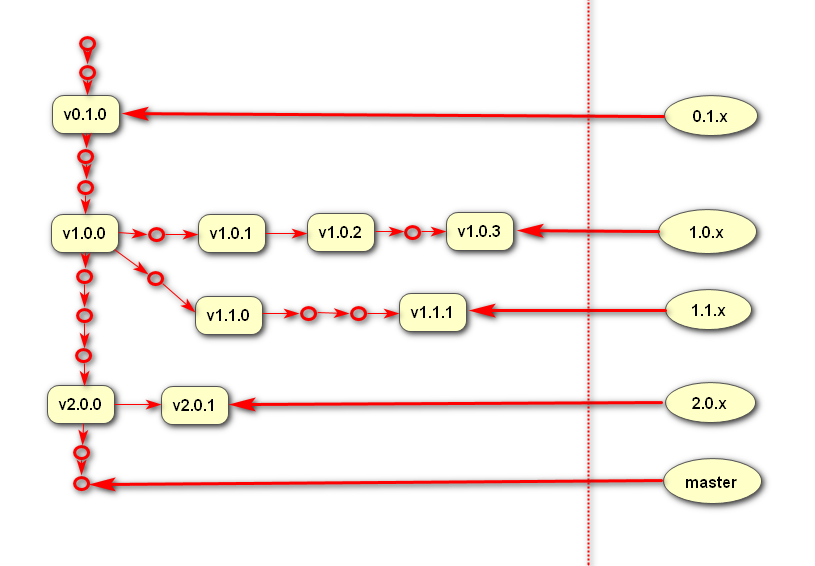
\includegraphics[width=\linewidth]{img/branches.png}
		\caption{Esempio di versionamento tramite l'utilizzo di \textit{branch}}
		\label{fig:branches}
	\end{figure}

	Quando si lavora su una repository condivisa è utile inoltre utilizzare i \textit{branch}, ovvero linee di sviluppo indipendenti che non vanno a interferire con il software in produzione.
	Tali branch possono essere utilizzati da una sola persona in maniera da non interferire con il lavoro di altri o da un team di persone.
	Nel caso in cui vi fossero errori nel branch, questi possono essere corretti senza che il resto del sistema ne sia influenzato.
	Ulteriormente, tali branch possono essere cancellati senza che il resto del sistema ne sia colpito.
	
	La Fig. \ref{fig:branches}~rappresenta sulla sinistra la linea di sviluppo tramite commit e branch mentre sulla destra le versioni attuali del sistema.
	
	Per i CI che rappresentano una versione MAJOR di una porzione di software, verrà utilizzato l'approccio \textit{PUSH}, ovvero la nuova versione viene mandata a tutti gli utilizzatori del sistema che dovranno installarla (a meno che l'installazione non avvenga automaticamente).
	Le versioni MINOR e PATCH verranno rilasciate secondo l'approccio \textit{PULL}, ovvero saranno gli utilizzatori del sistema a decidere il momento in cui effettuare il download e l'update alla nuova versione.
	In certi casi, come ad esempio il fix di un bug che compromette la sicurezza del sistema, queste potranno tuttavia essere rilasciate in modalità PUSH, obbligando dunque a installare subito la nuova versione.
	
\newpage
\section{Pianificazione dell'implementazione}\label{sec:pianificazione}

	Vengono quindi presentati in questa sezione tre diagrammi di Gantt, rappresentati in Fig. \ref{fig:anno_1}, Fig. \ref{fig:anno_2}~e Fig. \ref{fig:anno_3}, che servono come rappresentazione della pianificazone temporale del progetto.
	Per ciascuna attività vengono assegnate una \textit{data di inizio}, una \textit{data di fine} e una \textit{durata}.
	Si suppone che la firma del contratto e l'inizio del lavoro avvengano in data 1 Febbraio 2021.
		
	\subsection{\rollout~per settori sanitari}	
	
		Come accennato in \ref{sec:desc_implementazione}, il \rollout~viene effettuato verticalmente e per ciascun settore sanitario presente nella Fig. \ref{fig:gerarchia}~che rappresenta la gerarchia dell'\istituto.
		
		Per primo verrà implementato il \textit{backbone} del sistema, ovvero verrà revisionata l'architettura della rete.
		Questo verrà fatto partendo dalle connessioni principali, ovvero quelle che portano da e verso il Centro Elaborazione Dati, e successivamente per ciascuno dei dipartimenti.
		
		Non appena sarà disponibile una prima versione delle componenti software che compongono il progetto, queste verranno installate in ordine cronologico in ciascun dipartimento, in base ad una lista di priorità scelta tra \azienda~e \istituto.
		Con l'installazione del software verrà anche rinnovato l'hardware, sempre in maniera cronologica.
		
		A colmare il \textit{gap} che verrà a formarsi tra il nuovo sistema e il vecchio, nell'attesa che quest'ultimo venga totalmente dismesso, \azienda~si impegna a scrivere un software intermedio che possa mettere in comunicazione i due sistemi.
		Nonostante questo implichi un uso di risorse più elevato, è utile in caso di \rollback.
	
	\begin{sidewaysfigure}
		\centering
		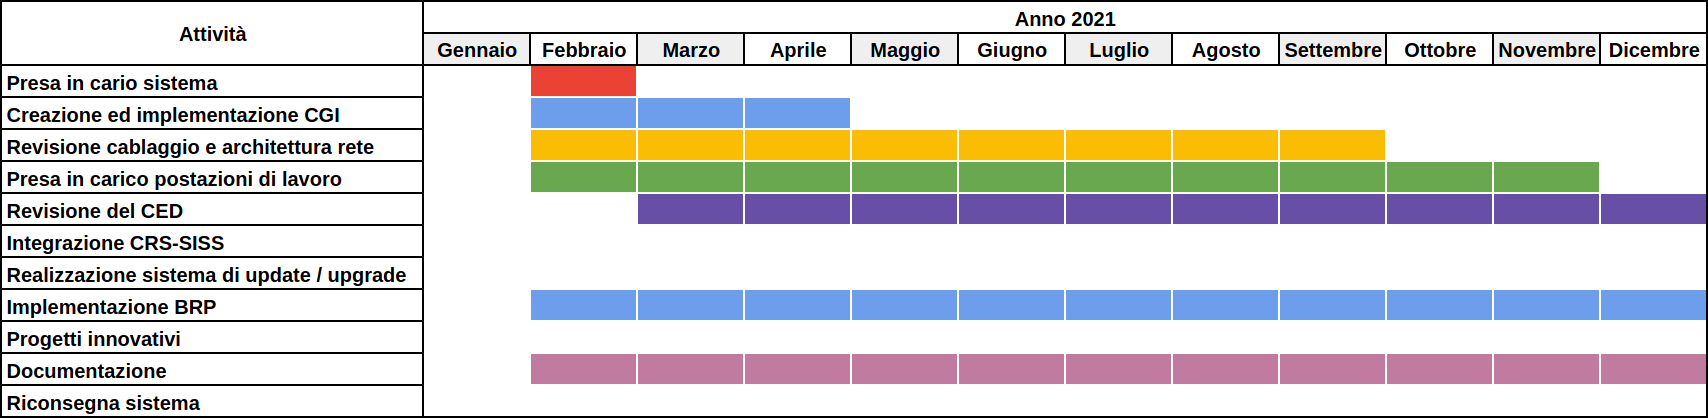
\includegraphics[width=\linewidth-2cm]{img/pianificazione_anno_1.png}
		\caption{Pianificazione sistema al primo anno}
		\label{fig:anno_1}
		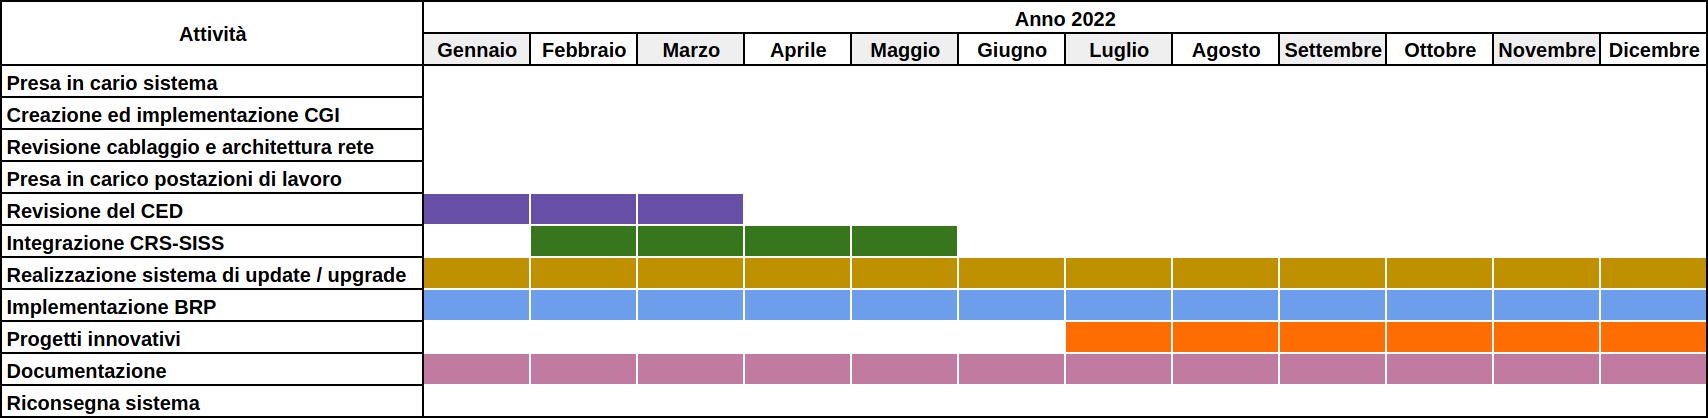
\includegraphics[width=\linewidth-2cm]{img/pianificazione_anno_2.png}
		\label{fig:anno_2}
		\caption{Pianificazione sistema al secondo anno}
		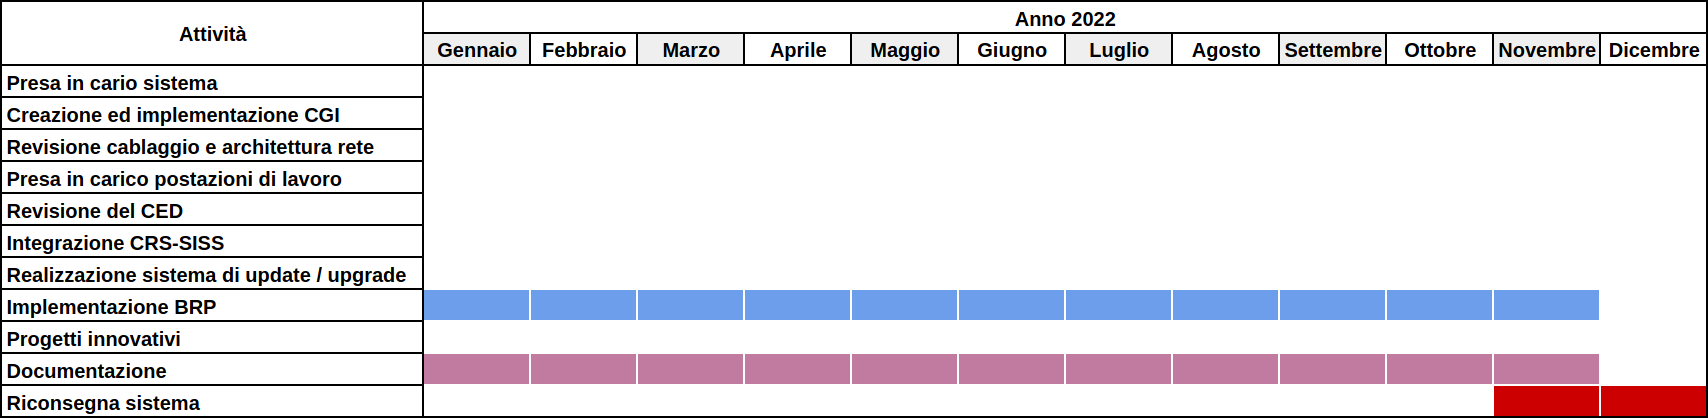
\includegraphics[width=\linewidth-2cm]{img/pianificazione_anno_3.png}
		\label{fig:anno_3}
		\caption{Pianificazione sistema al terzo anno}
	\end{sidewaysfigure}
	
%\newpage
\section{\rollback~del sistema}

	% https://everythingwhat.com/what-is-a-rollback-plan-in-change-management
	% A rollback plan is exactly what it sounds like. It's a list of steps you'd take to undo a release and restore the system to its original state. Writing a rollback plan can also help clarify what impact the release is expected to have on other systems and what other steps should be taken.

	Avere un piano di \rollback~è essenziale quando si pianifica l'implementazione di una nuova feature all'interno di un sistema.
	È quindi composto da una lista di passi da seguire per disfare o annullare quello che è stato introdotto, andando quindi a ripristinare il sistema al suo stato originario.
	
	Un piano di \rollback~ben definito può aiutare inoltre a chiarificare l'impatto che un upgrade o l'installazione di una nuova release ha sul sistema e in che modo questo ne viene influenzato.

	È quindi necessario creare un piano di \rollback~per ciascuna nuova versione del sistema.
	A questo scopo verranno messi a disposizione da \azienda~alcuni template della documentazione necessaria per fissare i passi da seguire in caso di \rollback.
	Questi variano in base al tipo di installazione che si viene a eseguire, ovvero in caso venga installato semplicemente una \textit{patch}, una \textit{minor release} o una \textit{major release}, come descritte in \ref{sec:configurazione}.

\newpage
\section{Criteri di accettazione}

	Per ciascuna attività, come quelle descritte in Sez. \ref{sec:attivita_principali}, vi sono alcuni \textit{criteri di accettazione} che ne decretano la corretta conclusione.

	Secondo il framework ITIL, l'accettazione (o \textit{validazione}) viene eseguita dal processo di \textit{Service Validation and Testing}, composto dai seguenti sottoprocessi:
	% TODO cambiare
	\begin{itemize}[noitemsep]
		\item \textit{Definizione del modello di test} (o \textit{Test Model Definition}): specifica in dettaglio come la release verrà testata, definendo i test case da utilizzare per la validazione; 
		\item \textit{Acquisizione delle componenti della release} (o \textit{Release Component Acquisition}): acquisisce le componenti di una release e valuta inizialmente, assicurandosi che solo le componenti che superano dei controlli di qualità stringenti possano essere testate in modo intensivo;
		\item \textit{Test della release} (o \textit{Release Test}): testa tutte le componenti e tutti gli strumenti e le tecniche richieste per l’implementazione, la migrazione e il back out di una release. Solo le componenti che superano questi test possono entrare nell’ambiente live;
		\item \textit{Test di accettazione del servizio} (o \textit{Service Acceptance Testing}): verifica che sussistano tutte le condizioni affinchè il servizio possa essere attivato e ottiene il consenso da parte dell’utente che il servizio rispetta gli SLA concordati.
	\end{itemize}
	
	\begin{figure}[h!]
		\centering
		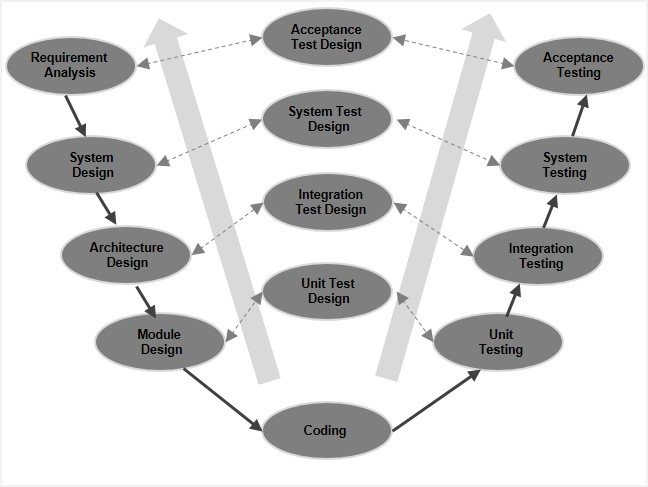
\includegraphics[width=\linewidth-2cm]{img/sdlc_v_model.jpeg}
		\caption{Modello a V\cite{vmodel}}
		\label{fig:vmodel}
	\end{figure}

	\azienda, come per altri progetti svolti in passato, ritiene opportuno utilizzare il ``\textit{Modello a V}'', rappresentato in Fig. \ref{fig:vmodel}, come approccio per la Verifica e Validazione.
	
	La validazione esterna, ovvero quella svolta attraverso i test di sistema insieme al propontente, è di importanza cruciale per \azienda.
	Per questo motivo viene data particolare attenzione a questi in quanto step finale per certificare la conformità complessiva del progetto.
	
	Tuttavia questa situazione non dovrebbe accadere in quanto verranno pianificati meeting quindicinnali insieme agli stakeholders per validare l'andamento del progetto.
	L'esito di tali meeting verrà salvato in documenti che conterranno i punti che sono stati trattati e gli interventi delle persone coinvolte.

\newpage
\section{Gestione dei rischi ed impatto}\label{sec:rischi}

	In questa sezione viene descritto come verranno catalogati i rischi ed i problemi che possono provocare danni al sistema, alle informazioni che questo contiene e, dunque, ai pazienti e ai dipendenti che lo utilizzano.
	
	Secondo il \textit{CRAMM} (``\textit{CCTA Risk Analysis and Management Method}''), il rischio si può definire come il prodotto tra valore dell'asset, minaccia e vulnerabilità.
	
	\begin{figure}[h!]
		\centering
		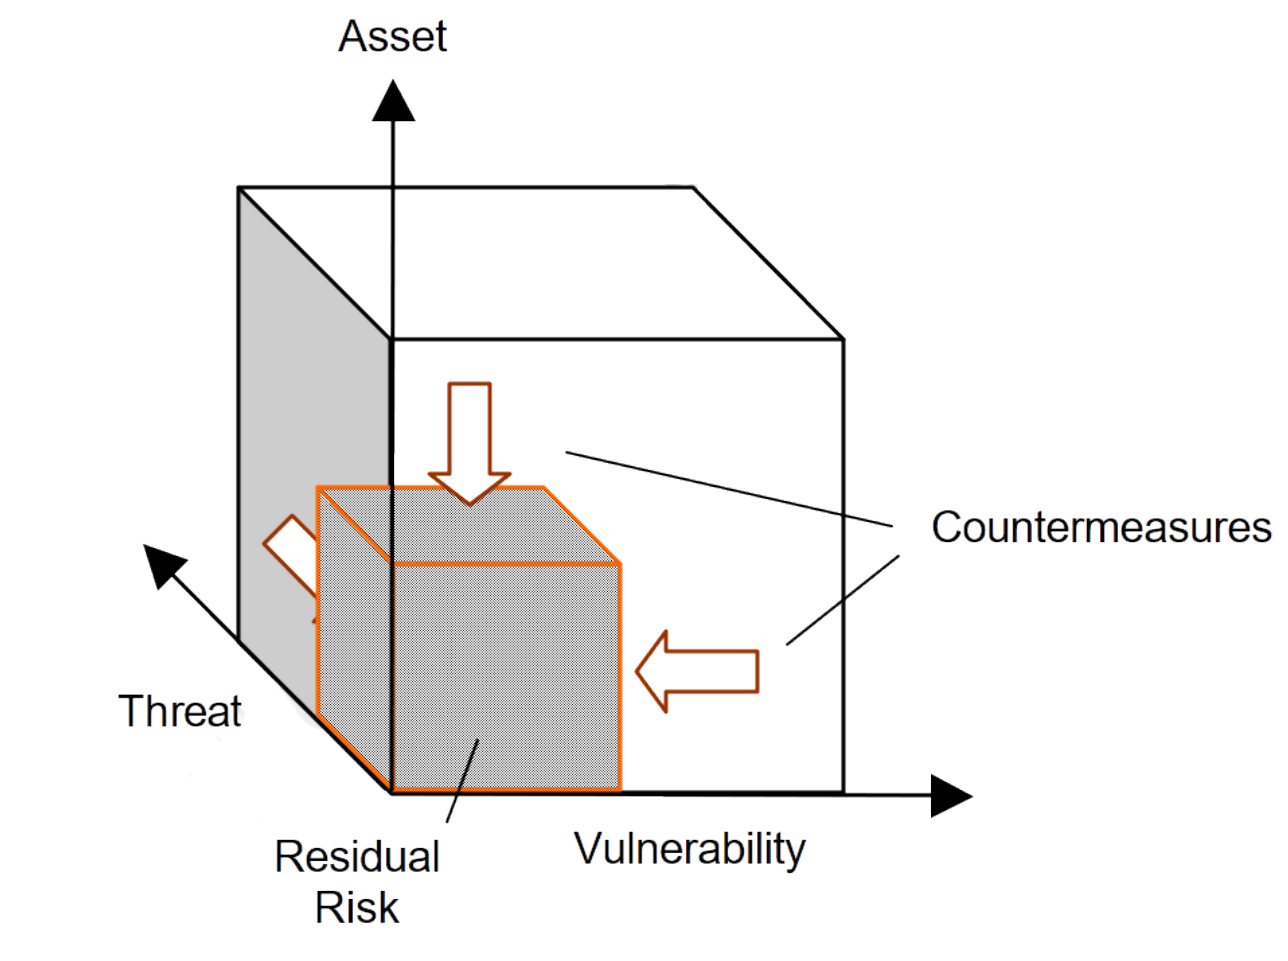
\includegraphics[width=\linewidth-2cm]{img/risk.png}
		\caption{Rappresentazione del rischio\cite{risk}}
		\label{fig:risk}
	\end{figure}

	Per stimare l'impatto dei rischi viene utilizzata la matrice ``\textit{probabilità-impatto}'' rappresentata in Fig. \ref{fig:risk_matrix}, dove livello di rischio viene calcolato come l'intersezione tra:
	\begin{itemize}[noitemsep]
		\item \textit{Probabilità}: la risposta alla domanda ``\textit{quanto è probabile che accada questo evento?}'';
		\item \textit{Impatto}: la risposta alla domanda ``\textit{quanto è sconvolgente questo evento sul sistema?}'';
	\end{itemize}
	Il rischio ha quindi una misura qualitativa che può avere questi valori:
	\begin{itemize}[noitemsep]
		\item \textit{Rischio molto basso}: tale evento ha un impatto minimo sul sistema e sui suoi utenti, è possibile rivolgerlo nella versione da rilasciare successivamente;
		\item \textit{Rischio basso}: tale evento può provocare sconforto nell'uso del sistema da parte degli utenti;
		\item \textit{Rischio moderato}: tale evento può risultare in un downtime del sistema e necessita di essere analizzato con cura;
		\item \textit{Rischio alto}: tale evento minaccia il sistema e deve essere risolto prima che accada;
		\item \textit{Rischio molto alto}: tale evento mette a repentaglio la sicurezza del sistema e dei suoi utenti risultando catastrofico per l'\istituto. 
		Va risolto immediatamente e tutto il sistema va aggiornato.
	\end{itemize}
	
	\begin{figure}[h!]
		\centering
		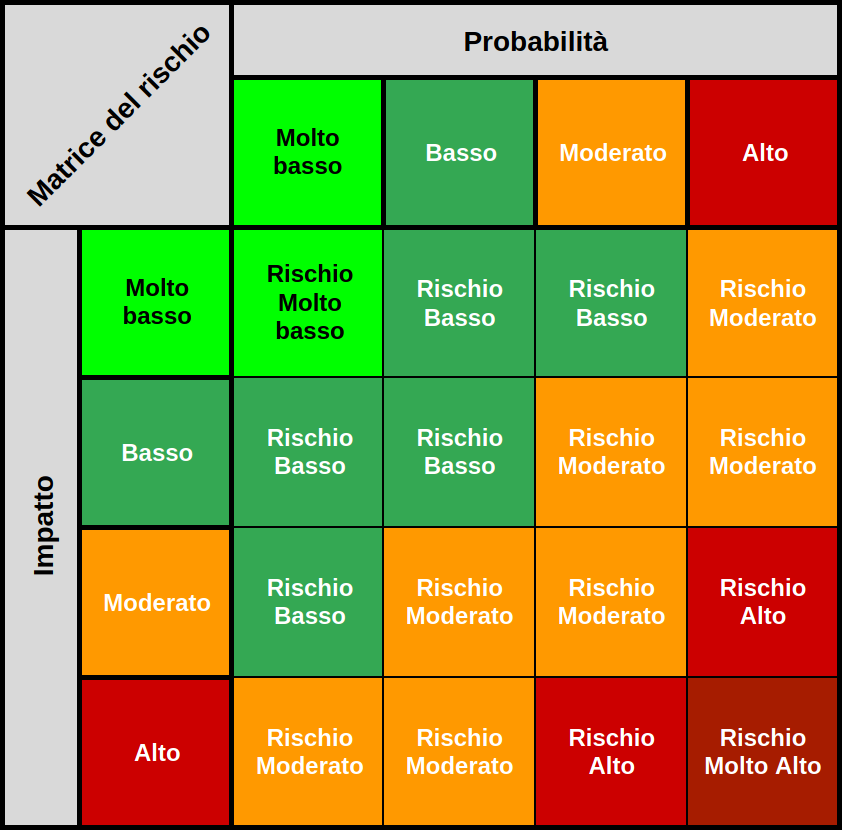
\includegraphics[width=\linewidth]{img/matrix.png}
		\caption{\textit{Risk Assessment Matrix}}
		\label{fig:risk_matrix}
	\end{figure}

	Un'analisi approfondita dei rischi sarà presentata nella documentazione riguardante il processo di ``\textit{Risk Management}''.

\newpage
\section{Privacy e sicurezza del sistema}

	\azienda~si impegna a garantire che il progetto svolto per l'\istituto~sia sicuro considerando gli standard della privacy e quelli della sicurezza.
	Per questo tali aspetti verranno trattati durante l'implementazione seguendo i principi di \textit{security by design}.

	\subsection{Privacy}
		
		Per tale aspetto, il regolamento principale su cui fare affidamento è quello del 
		``\textit{General Data Protection Regulation}'' (o \textit{GDPR}), rilasciato nella prima metà del 2018.
		Seguendo questo regolamento ci sono due aspetti fondamentali da considerare:
		\begin{itemize}
			
			\item il primo riguarda il consenso del soggetto di cui si stanno trattando i dati. 
			Questo deve essere sempre richiesto preventivamente e senza che possa essere equivoco;
			escludendo ogni ipotesi di consenso tacito.
			
			\item il secondo riguarda i casi di violazioni esterne (o ``\textit{data breach}'') quali furti di informazioni via Internet o fisicamente.
			Se dovesse presentarsi questa situazione, il responsabile del sistema, in quanto titolare del trattamento dei dati, dovrà preoccuparsi di communicare l'accaduto immediatamente ai proprietari dei dati e ad eventuali soggetti come ad esempio il garante nazionale o la polizia postale.
			
		\end{itemize}
		
	\subsection{Sicurezza}
	
		Al di là della privacy dei dati e dei processi, è necessario che il sistema sia sicuro da ogni altra prospettiva.
		Dal punto di vista \textit{ITIL}, la sicurezza (\textit{security}) è:
		\begin{itemize}[noitemsep]
			\item \textit{Confidentiality};
			\item \textit{Integrity};
			\item \textit{Availability}.
		\end{itemize}
	
		Questi tre componenti, che formano l'anagramma di \textit{CIA}, rispondono alle violazioni  del sistema con contenimenti e correzioni.
		
		I livelli di security che vengono descritti da ITIL si basano principalmente in ambito IT, ovvero sugli strumenti e sulle tecnologie, a differenza della privacy che ha un maggiore orientamento verso i processi.